\documentclass[11pt, a4paper]{article}

% --- Codificación y lenguaje ---
\usepackage[utf8]{inputenc}
\usepackage[T1]{fontenc}
\usepackage[spanish]{babel}

% --- Márgenes ---
\usepackage[margin=2.5cm]{geometry}

% --- Matemáticas ---
\usepackage{amsmath, amssymb}

% --- Tablas y figuras ---
\usepackage{graphicx}
\usepackage{booktabs}
\usepackage{array}
\usepackage{multirow}
\usepackage{caption}
\usepackage{subcaption}
\usepackage{float}

% --- Cajas de advertencia ---
\usepackage{xcolor}
\usepackage{tcolorbox}
\tcbuselibrary{breakable}

% --- Listas ---
\usepackage{enumitem}

% --- Hipervínculos ---
\usepackage[colorlinks=true, linkcolor=blue, citecolor=blue, urlcolor=blue]{hyperref}

% --- Códigos ---
\usepackage{listings}
\lstset{
  basicstyle=\ttfamily\footnotesize,
  breaklines=true,
  frame=single,
  xleftmargin=10pt,
  xrightmargin=10pt,
  showstringspaces=false,
}

% --- Caja de "advertencia" para confounds ---
\newtcolorbox{warningbox}[1][]{
  colback=red!5!white,
  colframe=red!75!black,
  fonttitle=\bfseries,
  title=#1,
  breakable,
}

% --- Encabezado ---
\title{
    \textbf{Informe final de proyecto:} \\[4pt]
    Replicación independiente del pipeline de Lopes et al.~(2023) sobre
    OpenNeuro \texttt{ds004504} y comparación STFT vs CWT-Morlet
    como etapa de descomposición tiempo-frecuencia
}
\author{
    Sebastián Palacio Betancur \\[6pt]
    \textit{Universidad Nacional de Colombia -- Sede Medellín} \\
    \textit{Facultad de Minas} \\[6pt]
    Curso: Tópicos en Procesamiento Digital de Señales \\
    Profesor: Freddy Bolaños
}
\date{Julio de 2026}

\begin{document}
\maketitle

% =============================================================
\section*{Resumen ejecutivo}
% =============================================================

Este trabajo replica de forma independiente el pipeline de Lopes
et al.~\cite{Lopes2023} (CNN sobre espectrograma de modulación de EEG
con saliency-guided patches + SVM) sobre el dataset público OpenNeuro
\texttt{ds004504}~\cite{Miltiadous2023} (65 sujetos: 36~AD + 29~HC), y
extiende el análisis comparando \textbf{STFT} y \textbf{CWT-Morlet}
como etapa de descomposición tiempo-frecuencia.

Las cifras principales se reportan como media~$\pm$~SD entre 3~semillas
de inicialización (LOSO-CV, 65~folds, anti-leakage estricto por fold en
preproceso, saliency y selección de features). Para separar el efecto de
la \textbf{transformada} del de un \textbf{artefacto de DSP} en el eje de
modulación (§3.3), se evalúan \textbf{tres} representaciones
tiempo-frecuencia: STFT, CWT-Morlet nativa, y \textbf{CWT-fair} (CWT con
la envolvente decimada para igualar el eje de modulación de la STFT ---
misma resolución de modulación, distinta resolución de portadora).

\begin{table}[H]
\centering
\small
\begin{tabular}{llccc}
\toprule
Clasificador & T-F & Acc & F1 macro & AUC \\
\midrule
SVM vainilla (paper-faithful) & \textbf{STFT} &
  $\mathbf{0.764 \pm 0.009}$ & $\mathbf{0.762 \pm 0.011}$ & $\mathbf{0.856 \pm 0.022}$ \\
SVM vainilla & CWT nativa &
  $0.677 \pm 0.081$ & $0.673 \pm 0.094$ & $0.778 \pm 0.038$ \\
SVM vainilla & \textbf{CWT-fair} &
  $0.754 \pm 0.046$ & $0.750 \pm 0.046$ & $\mathbf{0.828 \pm 0.031}$ \\
SVM Grad-CAM & STFT &
  $0.662 \pm 0.031$ & $0.643 \pm 0.041$ & $0.713 \pm 0.020$ \\
SVM Grad-CAM & CWT nativa &
  $0.703 \pm 0.009$ & $0.687 \pm 0.026$ & $0.800 \pm 0.010$ \\
SVM Grad-CAM & \textbf{CWT-fair} &
  $0.682 \pm 0.054$ & $0.673 \pm 0.050$ & $0.769 \pm 0.045$ \\
CNN end-to-end & STFT &
  $0.656 \pm 0.024$ & $0.642 \pm 0.020$ & $0.695 \pm 0.022$ \\
CNN end-to-end & CWT nativa &
  $0.626 \pm 0.071$ & $0.611 \pm 0.070$ & $0.590 \pm 0.069$ \\
CNN end-to-end & \textbf{CWT-fair} &
  $0.656 \pm 0.062$ & $0.655 \pm 0.061$ & $0.667 \pm 0.067$ \\
\bottomrule
\end{tabular}
\caption{Resultados globales por configuración (3~seeds, LOSO-CV 65~folds).}
\label{tab:resumen}
\end{table}

\noindent\textbf{Conclusiones clave (con matices estadísticos explícitos)}:

\begin{enumerate}[leftmargin=*]
    \item \textbf{La replicación independiente del pipeline funciona}:
    SVM con saliency vainilla y STFT alcanza
    Acc $0.764 \pm 0.009$, AUC $0.856 \pm 0.022$, en el rango del
    $0.71 \pm 0.02$ reportado por Lopes (T2: N vs AD).
    La comparación es orientativa, no equivalencia estricta.

    \item \textbf{Las diferencias aparentes STFT vs CWT eran en gran
    parte un artefacto de DSP, no de la transformada.} El eje de
    modulación de la STFT (Nyquist 1.56~Hz) y el de la CWT nativa
    (Nyquist 100~Hz) NO codifican el mismo contenido antes del resize
    a $45\times45$. Al igualarlos (CWT-fair), la brecha con STFT se
    reduce a la mitad o más en ambos métodos de saliency: con vainilla
    la CWT pasa de $-0.078$ AUC a $\mathbf{-0.028}$; con Grad-CAM de
    $+0.087$ a $\mathbf{+0.056}$. Igualar el eje \textbf{mueve la CWT
    hacia la STFT en las dos direcciones}.

    \item \textbf{Con el eje de modulación igualado, STFT y CWT son
    estadísticamente indistinguibles.} DeLong por seed + Stouffer:
    STFT vs CWT-fair $p = 0.318$ (vainilla), $0.587$ (Grad-CAM); CWT
    nativa vs CWT-fair $p = 0.283$, $0.527$. Ninguna comparación es
    significativa. \textbf{La elección STFT vs CWT-Morlet no cambia el
    desempeño de este pipeline una vez controlado el eje}; ni la
    hipótesis original (CWT > STFT) ni la inversa obtienen evidencia.

    \item \textbf{El método de saliency afecta el ranking aparente entre
    STFT y CWT nativa} (Grad-CAM: CWT mejor; vainilla: STFT mejor), pero
    esa sensibilidad \textbf{se atenúa con CWT-fair}: buena parte del
    ``cambio de ranking'' también era el artefacto DSP.

    \item \textbf{Análisis exploratorio (post-hoc)}: STFT~+~vainilla
    concentra $\sim$89\% de la saliency en bandas $\alpha$~(61\%)~+
    $\theta$~(28\%) y canales occipito-temporales (O1, O2, T5, T6),
    coherente con literatura clínica EEG-AD.
\end{enumerate}

% =============================================================
\section{Introducción}
% =============================================================

\subsection{Contexto clínico}

La enfermedad de Alzheimer (EA) es la causa más común de demencia, con
más de 55~millones de personas afectadas globalmente. El diagnóstico
temprano es crítico para la intervención terapéutica. Las técnicas
estándar de imagen (RM, PET) son costosas y poco accesibles. El EEG
es no invasivo, portátil y económico, lo cual lo posiciona como
herramienta promisoria para tamizaje a escala poblacional.

\subsection{Espectrograma de modulación}

El \emph{espectrograma de modulación} del EEG captura periodicidades
de segundo orden: cómo varía temporalmente la energía de cada
componente espectral. Formalmente, dada una representación
tiempo-frecuencia $X(t,f)$:

\begin{equation}
    M(f, f_m) = \mathcal{F}_t \left\{ |X(t,f)|^2 \right\}
    \label{eq:modspec}
\end{equation}

\noindent donde $f$ es la frecuencia portadora y $f_m$ la frecuencia
de modulación. Trambaiolli~\cite{Trambaiolli2011},
Fraga~\cite{Fraga2013}, Cassani~\cite{Cassani2020} y
Lopes~\cite{Lopes2023} han demostrado consistentemente que esta
representación captura biomarcadores discriminativos de EA.

\subsection{Trabajo de referencia: Lopes et al.~2023}

Lopes et al.~\cite{Lopes2023} propusieron entrenar una CNN sobre el
espectrograma de modulación y usar \textbf{mapas de saliencia} (vanilla
gradient) para descubrir regiones discriminativas (``patches''). Sobre
estos patches calculan potencia~+~ratios como features para un SVM
final. Reportan accuracy $\sim 0.71$ en LOSO-test sobre $N=39$~sujetos
de un dataset privado.

\subsection{Objetivos}

\begin{enumerate}[leftmargin=*]
    \item \textbf{Validar de forma independiente} el pipeline de Lopes
    sobre el dataset público OpenNeuro \texttt{ds004504}.
    \item \textbf{Comparar STFT vs CWT-Morlet} como etapa de
    descomposición tiempo-frecuencia.
    \item \textbf{Cuantificar la varianza por seed} con multi-seed
    LOSO-CV (3~seeds).
    \item \textbf{Analizar la interpretabilidad} de los patches
    descubiertos en términos de bandas canónicas y canales.
\end{enumerate}

\subsection{Pregunta de investigación}

\begin{quote}
\itshape ¿Produce la sustitución de la STFT por la CWT con wavelet de
Morlet un espectrograma de modulación con mayor poder discriminativo
para EA, y revela regiones de saliencia distintas a las reportadas por
Lopes et al.?
\end{quote}

% =============================================================
\section{Datos}
% =============================================================

\textbf{OpenNeuro \texttt{ds004504}}~\cite{Miltiadous2023}:
88~sujetos con EEG en reposo (ojos cerrados):

\begin{table}[H]
\centering
\small
\begin{tabular}{lccc}
\toprule
Grupo & $N$ & Edad (media~$\pm$~SD) & MMSE \\
\midrule
\textbf{A} (Alzheimer, AD) & 36 & $66.4 \pm 7.9$ & $17.8 \pm 4.5$ \\
\textbf{C} (Healthy Control, HC) & 29 & $67.9 \pm 5.4$ & $30.0 \pm 0.0$ \\
F (Frontotemporal Dementia) & 23 & --- & --- \\
\bottomrule
\end{tabular}
\caption{Composición del dataset \texttt{ds004504}.}
\end{table}

Este TFM utiliza solo los grupos \textbf{A y C} (clasificación binaria
AD vs HC, 65~sujetos). El grupo F (FTD) se excluyó del análisis
principal.

\textbf{Características técnicas}:
\begin{itemize}[leftmargin=*]
    \item 19~canales 10-20 (Fp1, Fp2, F3, F4, C3, C4, P3, P4, O1, O2,
    F7, F8, T3, T4, T5, T6, Fz, Cz, Pz).
    \item Frecuencia de muestreo nativa: 500~Hz $\rightarrow$
    resampleada a 200~Hz (alineación con Lopes).
    \item Duración registros: $\sim$10--13~min por sujeto.
    \item Licencia: CC0~1.0.
\end{itemize}

\textbf{Análisis de confounders (AD vs HC)}:

\begin{table}[H]
\centering
\small
\begin{tabular}{lcccc}
\toprule
Variable & AD & HC & Test & $p$ \\
\midrule
Edad             & $66.4 \pm 7.9$ & $67.9 \pm 5.4$ & $t$-test & $0.384$ (NS) \\
MMSE             & $17.8 \pm 4.5$ & $30.0 \pm 0.0$ & $t$-test & $<0.001$ (esperado) \\
Género (F/M)     & 24/12 & 11/18 & $\chi^2$ & $\mathbf{0.039}$ (SIG) \\
\bottomrule
\end{tabular}
\caption{Confounders demográficos. Existe sesgo significativo de género
en el dataset, discutido en §5.4 y §5.5.}
\end{table}

% =============================================================
\section{Pipeline implementado}
% =============================================================

\subsection{Preproceso EEG}

\begin{enumerate}[leftmargin=*]
    \item \textbf{Re-referencia}: promedio común (CAR).
    \item \textbf{Filtro pasa-banda}: FIR fase cero, 0.5--45~Hz.
    \item \textbf{Eliminación de artefactos}: ICA Infomax +
    ICLabel~\cite{PionTonachini2019} (rechazo de componentes con
    prob~$\geq 0.8$ para \emph{eye blink}, \emph{muscle artifact},
    \emph{heart beat}, \emph{line noise}, \emph{channel noise}).
    Desviación respecto al paper: Lopes usa wICA; ICLabel es una
    alternativa reproducible y estándar en MNE-Python.
    \item \textbf{Resample} a 200~Hz.
    \item \texttt{anonymize(daysback=10000)}.
\end{enumerate}

\subsection{Epoching}

\begin{itemize}[leftmargin=*]
    \item Duración: 8~s, paso 1~s (overlap 7~s) $\rightarrow$
    $\sim$470~epochs/sujeto.
    \item Descarte de los últimos 7~s para evitar leakage entre folds.
\end{itemize}

\subsection{Espectrograma de modulación}

\begin{itemize}[leftmargin=*]
    \item \textbf{STFT}: ventana Hann, \texttt{nperseg=128},
    \texttt{noverlap=64} a $f_s = 200$~Hz.
    \begin{itemize}
        \item Resolución frecuencial portadora real:
        $\Delta f = f_s / \texttt{nperseg} = 1.5625$~Hz
        (no 1~Hz nominal).
        \item Frecuencia de muestreo de la envolvente
        (eje temporal de la FFT de modulación):
        $dt = \texttt{noverlap}/f_s = 0.32$~s $\Rightarrow$
        Nyquist de modulación $= 1.5625$~Hz.
    \end{itemize}
    \item \textbf{CWT-Morlet nativa} (\texttt{cmor1.5-1.0}, 32~escalas
    log en $[0.5, 45]$~Hz):
    \begin{itemize}
        \item Frecuencia de muestreo de la envolvente: 200~Hz
        (CWT preserva $f_s$) $\Rightarrow$
        Nyquist de modulación $= 100$~Hz, $\sim$180~bins
        disponibles en $[0, 22.5]$~Hz.
    \end{itemize}
    \item \textbf{CWT-fair} (misma CWT-Morlet, misma portadora): la
    envolvente de potencia se \textbf{decima a 3.125~Hz} (anti-alias
    poly-phase FIR) \emph{antes} de la FFT temporal, igualando el
    Nyquist de modulación de la STFT (1.5625~Hz, $\sim$13~bins reales).
    Solo cambia el eje de modulación; la descomposición de portadora
    (wavelet, 32~escalas) es idéntica a la CWT nativa.
    \item \textbf{Procesamiento común}: $|X|^2 \rightarrow$ FFT
    temporal $\rightarrow$ recorte ($[0.5, 45]$~Hz portadora,
    $[0, 22.5]$~Hz modulación) $\rightarrow$ resize bilinear a
    $45\times45$ $\rightarrow$ log-power.
\end{itemize}

\begin{warningbox}[Asimetría de DSP en el eje de modulación --- y cómo se controla]
Las imágenes ``$45 \times 45$'' de STFT y CWT nativa \textbf{NO
representan el mismo rango físico del eje de modulación}:
\begin{itemize}[leftmargin=*, topsep=2pt]
    \item STFT: 0 a $\mathbf{1.5625}$~Hz (interpolado de 13~bins reales a 45 vía bilineal).
    \item CWT nativa: 0 a $\mathbf{22.5}$~Hz (subsampleado de $\sim$180~bins a 45).
\end{itemize}
Por tanto, una comparación STFT vs CWT nativa mezcla dos efectos: la
\textbf{transformada} (resolución de portadora) y la \textbf{resolución
del eje de modulación}. Para separarlos se introduce \textbf{CWT-fair},
que mantiene la transformada CWT pero iguala el eje de modulación al de
la STFT. Así:
\begin{itemize}[leftmargin=*, topsep=2pt]
    \item \textbf{STFT vs CWT-fair} aísla el efecto de la transformada a
    igualdad de eje (comparación justa).
    \item \textbf{CWT nativa vs CWT-fair} cuantifica el artefacto de DSP.
\end{itemize}
Resultado (§4.3): ambas comparaciones son \textbf{no significativas} ---
la asimetría de DSP explica la mayor parte de las diferencias aparentes
STFT$\leftrightarrow$CWT. \\
\textbf{Nota}: CWT-fair ``iguala hacia abajo'' (descarta las
modulaciones rápidas de la CWT). Es fisiológicamente defendible (la AM
diagnóstica en EA es lenta, $<2$~Hz; Fraga 2013), pero es una de dos
definiciones de ``justo''; la alternativa (subir la STFT con hop fino)
se deja como trabajo futuro (§5.5).
\end{warningbox}

\subsection{CNN — réplica de la arquitectura del paper}

\begin{table}[H]
\centering
\small
\begin{tabular}{ll}
\toprule
Capa & Detalle \\
\midrule
Input & $(19, 45, 45)$ \\
Conv2D \#1 & 32~filtros, $3\times3$, ReLU, padding 1 \\
Dropout~2D & $0.85$ \\
MaxPool & $2\times2$ \\
Conv2D \#2 & 64~filtros, $3\times3$, ReLU, padding 1 \\
Dropout~2D & $0.85$ \\
MaxPool & $2\times2$ \\
Flatten + FC\#1 & 128~unidades, LeakyReLU$(0.1)$, Dropout 0.85 \\
FC\#2 & 64~unidades, LeakyReLU$(0.1)$, Dropout 0.85 \\
FC\#3 (output) & 2~clases (AD/HC) \\
\bottomrule
\end{tabular}
\caption{Arquitectura CNN replicada de Lopes et al.~2023.}
\end{table}

\begin{itemize}[leftmargin=*]
    \item \textbf{Optimizer}: NAdam, lr=$10^{-4}$,
    weight\_decay=$10^{-2}$ ($L_2$ del paper).
    \item \textbf{Batch size}: 128 (la GPU permite mayor que el batch~4
    del paper; resultados estables).
    \item \textbf{Epochs}: 50 con \emph{early stopping} (paciencia~10)
    sobre F1~macro de val.
    \item \textbf{AMP} (mixed precision) en GPU.
    \item \textbf{Class weights} balanceados.
\end{itemize}

\subsection{Saliency por fold (anti-leakage estricto)}

Para cada fold del LOSO:

\begin{enumerate}[leftmargin=*]
    \item Cargar el modelo entrenado en ese fold.
    \item Para cada sujeto de train del fold (subset estratificado
    de~20):
    \begin{itemize}
        \item \textbf{Grad-CAM}~\cite{Selvaraju2017} sobre la última
        conv $\rightarrow$ mapa $45\times45$ por clase.
        \item O bien \textbf{vainilla saliency}~\cite{Simonyan2014}
        — paper-faithful — gradiente $|\partial y / \partial x|$.
    \end{itemize}
    \item Promediar por clase $\rightarrow$ \texttt{saliency\_AD},
    \texttt{saliency\_HC}.
    \item \texttt{saliency\_diff} = \texttt{saliency\_AD} $-$
    \texttt{saliency\_HC}.
    \item Selección heurística de threshold/$K$ por fold sobre
    threshold $\in \{80, 82, \dots, 96\}$\% y $K \in \{3, 4, 5\}$ para
    KMeans $\rightarrow$ patches por fold.

    \emph{Nota metodológica}: la implementación efectiva (en
    \texttt{scripts/04\_extract\_saliency\_features.py}) maximiza la
    separabilidad de la saliency map (max contraste AD vs HC sobre
    píxeles candidatos), NO una validación nested con SVM en val set.
    Se discute como limitación.
\end{enumerate}

\subsection{SVM con patches saliency-guided}

\begin{enumerate}[leftmargin=*]
    \item Por epoch y canal: feature $=$ potencia media en cada
    patch $+$ ratios de potencia entre patches del mismo canal.
    \item \textbf{Selección}: ANOVA $F$-value top-24 sobre train.
    \item \textbf{MinMaxScaler} a $[-1, 1]$.
    \item \textbf{SVM RBF} con $\gamma = 1/24$, $C = 1$, sin tuning
    (alineado con Lopes).
\end{enumerate}

\subsection{Validación}

\begin{itemize}[leftmargin=*]
    \item \textbf{LOSO-CV} estricta con 65~folds.
    \item En cada fold, 1~sujeto adicional retenido para validación
    (early stopping).
    \item Z-score por canal con estadísticos SOLO de train.
    \item Saliency, patches y \texttt{SelectKBest} \textbf{por fold}
    (anti-leakage).
    \item 3~semillas (s0, s1, s2) por configuración $\rightarrow$
    reportar media~$\pm$~SD.
\end{itemize}

% =============================================================
\section{Resultados}
% =============================================================

Cada tabla compara las \textbf{tres} representaciones T-F: STFT, CWT
nativa y CWT-fair (CWT con el eje de modulación igualado a la STFT,
§3.3).

\subsection{CNN end-to-end (3 seeds)}

\begin{table}[H]
\centering
\small
\begin{tabular}{lccc}
\toprule
T-F & Acc & F1 macro & AUC \\
\midrule
STFT & $0.656 \pm 0.024$ & $0.642 \pm 0.020$ & $0.695 \pm 0.022$ \\
CWT nativa & $0.626 \pm 0.071$ & $0.611 \pm 0.070$ & $0.590 \pm 0.069$ \\
\textbf{CWT-fair} & $0.656 \pm 0.062$ & $0.655 \pm 0.061$ & $\mathbf{0.667 \pm 0.067}$ \\
\bottomrule
\end{tabular}
\caption{CNN end-to-end, multi-seed.}
\end{table}

Igualar el eje de modulación \textbf{recupera la mayor parte del déficit
de la CWT} también en la CNN: AUC pasa de 0.590 (nativa) a 0.667 (fair),
acercándose a STFT (0.695). La CNN sola opera cerca del baseline trivial
(0.554), coherente con su rol de extractor (no clasificador final) y su
dropout~0.85.

\subsection{SVM con patches Grad-CAM (3 seeds)}

\begin{table}[H]
\centering
\small
\begin{tabular}{lccc}
\toprule
T-F & Acc & F1 & AUC \\
\midrule
STFT & $0.662 \pm 0.031$ & $0.643 \pm 0.041$ & $0.713 \pm 0.020$ \\
CWT nativa & $\mathbf{0.703 \pm 0.009}$ & $\mathbf{0.687 \pm 0.026}$ & $\mathbf{0.800 \pm 0.010}$ \\
CWT-fair & $0.682 \pm 0.054$ & $0.673 \pm 0.050$ & $0.769 \pm 0.045$ \\
\bottomrule
\end{tabular}
\caption{SVM saliency Grad-CAM, multi-seed.}
\end{table}

Con Grad-CAM, la CWT \textbf{nativa} parecía la mejor (0.800). Pero al
igualar el eje de modulación, CWT-fair baja a 0.769 ---
\textbf{acercándose a STFT}. La ventaja aparente de la CWT nativa era en
parte el eje de modulación más rico, no la transformada. DeLong por seed
(Stouffer): STFT vs CWT-fair $p = 0.587$; CWT nativa vs CWT-fair
$p = 0.527$ --- ambas NS.

\subsection{SVM saliency vainilla (paper-faithful) — resultado principal}

\begin{table}[H]
\centering
\small
\begin{tabular}{lccc}
\toprule
T-F & Acc & F1 & AUC \\
\midrule
\textbf{STFT} & $\mathbf{0.764 \pm 0.009}$ & $\mathbf{0.762 \pm 0.011}$ & $\mathbf{0.856 \pm 0.022}$ \\
CWT nativa & $0.677 \pm 0.081$ & $0.673 \pm 0.094$ & $0.778 \pm 0.038$ \\
\textbf{CWT-fair} & $0.754 \pm 0.046$ & $0.750 \pm 0.046$ & $\mathbf{0.828 \pm 0.031}$ \\
\bottomrule
\end{tabular}
\caption{SVM saliency vainilla, multi-seed. Mejor AUC individual: STFT.}
\label{tab:svm_vanilla}
\end{table}

\subsubsection{Comparación justa: DeLong por seed + combinación}
\label{sec:delong_per_seed}

DeLong AUC pareado \emph{dentro de cada seed} (n=65 por test LOSO),
combinado entre seeds con Stouffer/Fisher. Se reportan tres
comparaciones:

\begin{table}[H]
\centering
\small
\begin{tabular}{lccl}
\toprule
Comparación & $\Delta$ AUC por seed & Stouffer $p$ & Lectura \\
\midrule
STFT vs CWT \textbf{nativa} (confundida) & $+0.028, +0.105, +0.101$ & $\mathbf{0.061}$ & marginal --- mezcla transformada + eje \\
\textbf{STFT vs CWT-fair} (justa) & $-0.021, +0.036, +0.069$ & $\mathbf{0.318}$ & NS --- sin diferencia a igualdad de eje \\
CWT nativa vs CWT-fair (efecto eje) & $-0.049, -0.069, -0.032$ & $\mathbf{0.283}$ & NS --- el eje explica el grueso \\
\bottomrule
\end{tabular}
\end{table}

\textbf{Interpretación}: la ventaja marginal de STFT sobre la CWT nativa
($p = 0.061$) \textbf{se disuelve a $p = 0.318$ cuando se iguala el eje
de modulación} (STFT vs CWT-fair). Ese $p \approx 0.06$ estaba impulsado
por el artefacto de DSP, no por la transformada. La CWT-fair recupera la
brecha ($0.778 \to 0.828$ AUC, $-0.078 \to -0.028$ vs STFT).
\textbf{A igualdad de eje de modulación, STFT y CWT-Morlet son
estadísticamente indistinguibles.}

\begin{figure}[H]
    \centering
    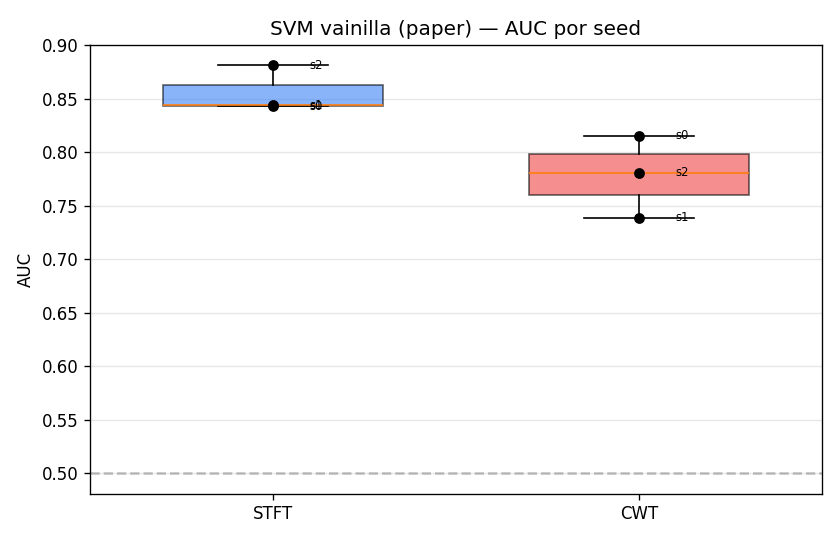
\includegraphics[width=0.9\textwidth]{figures_informe_final/svm_vanilla_auc_boxplot.png}
    \caption{Distribución de AUC por sujeto-test (LOSO) para SVM
    vainilla, agregada a través de 3~seeds.}
    \label{fig:svm_vanilla_boxplot}
\end{figure}

\begin{figure}[H]
    \centering
    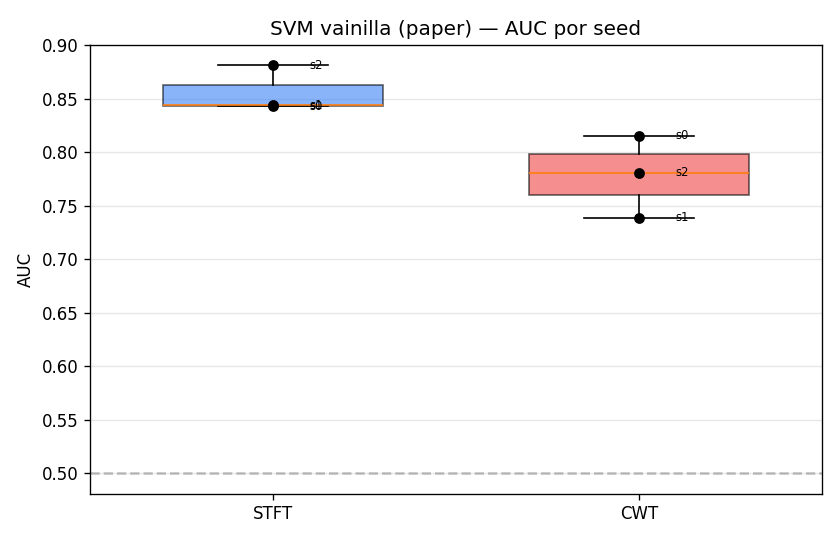
\includegraphics[width=0.9\textwidth]{figures_informe_final/svm_vanilla_auc_boxplot.png}
    \caption{Distribución de AUC por sujeto-test (LOSO) para SVM
    vainilla con STFT y CWT, agregada a través de 3~seeds. La
    superposición entre ambas distribuciones es coherente con la
    inferencia $p \approx 0.06$ (NS).}
    \label{fig:svm_vanilla_boxplot}
\end{figure}

\subsubsection{Corrección por múltiples comparaciones (BH-FDR)}
\label{sec:bhfdr}

Corrección Benjamini-Hochberg ($\alpha=0.05$) sobre los $p$-values
combinados (Stouffer) de las comparaciones \textbf{justas} STFT vs
CWT-fair (las que aíslan la transformada):

\begin{table}[H]
\centering
\small
\begin{tabular}{lccc}
\toprule
Comparación justa (STFT vs CWT-fair) & $p$ (Stouffer) & BH-FDR $q$ & Sig. \\
\midrule
SVM vainilla & $0.318$ & $0.587$ & \texttimes \\
SVM Grad-CAM & $0.587$ & $0.587$ & \texttimes \\
CNN & $0.266$ & $0.587$ & \texttimes \\
\bottomrule
\end{tabular}
\end{table}

\textbf{Ninguna comparación justa se acerca a la significancia}
($q \geq 0.58$). Incluso la comparación \emph{confundida} STFT vs CWT
nativa ($p=0.061$ vainilla, $0.068$ Grad-CAM) no sobrevivía BH-FDR
($q\approx0.10$); las justas están mucho más lejos. \textbf{A igualdad
de eje de modulación, no hay evidencia de superioridad de ninguna
transformada T-F en este pipeline.}

\subsubsection{Wilcoxon por seed individual (consistencia)}

Wilcoxon pareado de scores por sujeto en cada seed (SVM vainilla, STFT
vs CWT nativa) corrobora la falta de un efecto consistente incluso en la
comparación confundida:

\begin{center}
\small
\begin{tabular}{cc}
\toprule
seed & Wilcoxon $p$ \\
\midrule
$s_0$ & $0.893$ (NS) \\
$s_1$ & $0.025$ (sig. sin corregir) \\
$s_2$ & $0.338$ (NS) \\
\bottomrule
\end{tabular}
\end{center}

Solo en $s_1$ hay diferencia significativa, perdida tras Bonferroni
intra-seed ($\alpha = 0.0167$). La señal no se replica entre semillas.

\subsection{Comparación con el paper Lopes 2023}

\begin{table}[H]
\centering
\small
\begin{tabular}{lcc}
\toprule
Métrica & Paper Lopes (T2: N vs AD, LOSO test) & Este TFM (SVM vainilla STFT, 3 seeds) \\
\midrule
$N$ sujetos & 39 (20 N + 19 AD1) & 65 (29 HC + 36 AD) \\
Accuracy & $0.71 \pm 0.02$ & $\mathbf{0.764 \pm 0.009}$ \\
F1       & $0.61 \pm 0.02$ & $\mathbf{0.762 \pm 0.011}$ \\
AUC      & no reportado    & $\mathbf{0.856 \pm 0.022}$ \\
\bottomrule
\end{tabular}
\caption{Comparación con paper original. La comparación es orientativa;
no equivalencia estricta (datasets, poblaciones y anti-leakage difieren).}
\end{table}

El TFM obtiene cifras en el rango del paper o ligeramente superiores.
Lo defendible es que \textbf{el pipeline funciona en el mismo orden de
magnitud sobre datos públicos independientes}, que es el objetivo
principal de un estudio de replicación.

\subsection{Análisis de saliency: correlación 2D entre métodos}

\begin{table}[H]
\centering
\small
\begin{tabular}{lc}
\toprule
Comparación & Pearson $r$ (3 seeds, media $\pm$ SD) \\
\midrule
STFT vs CWT con Grad-CAM   & $-0.237 \pm 0.119$ \\
STFT vs CWT con vainilla   & $-0.086 \pm 0.076$ \\
Grad-CAM vs vainilla (STFT) & $+0.114 \pm 0.043$ \\
Grad-CAM vs vainilla (CWT)  & $-0.166 \pm 0.106$ \\
\bottomrule
\end{tabular}
\end{table}

\textbf{Interpretación}: los saliency maps STFT y CWT son
\textbf{estadísticamente ortogonales} (Pearson $r \approx -0.09$
vainilla, $-0.24$ Grad-CAM; ningún $p < 0.05$ para $r \neq 0$). Hablar
de ``anti-correlación'' sería sobreinterpretar el signo: las
correlaciones son estadísticamente indistinguibles de cero. Lo mismo
ocurre entre Grad-CAM y vainilla. Esto demuestra que ``el biomarcador
descubierto'' depende fuertemente de la elección de pipeline.

\subsection{Análisis por banda canónica (post-hoc, solo STFT)}

\begin{warningbox}[Restricción del análisis a STFT]
El eje de la portadora de la CWT está log-espaciado (\texttt{geomspace}),
por lo que la asignación píxel~$\to$~banda canónica difiere de la de la
STFT (\texttt{linspace}). El análisis aquí se restringe a STFT
(eje lineal nativo); para CWT requeriría reescribir el mapeo en el
script de post-experimentos.
\end{warningbox}

Proporción de píxeles top-10\% saliency en cada banda canónica
(media entre seeds):

\begin{table}[H]
\centering
\small
\begin{tabular}{lccccc}
\toprule
Configuración & $\delta$ (0.5--4) & $\theta$ (4--8) & $\alpha$ (8--13) & $\beta$ (13--30) & $\gamma$ (30--45) \\
\midrule
\textbf{STFT vainilla} & 5.8\% & $\mathbf{27.9\%}$ & $\mathbf{61.1\%}$ & 5.3\% & 0.0\% \\
STFT Grad-CAM & 0.0\% & 0.0\% & 0.0\% & 0.7\% & 99.3\% \\
\bottomrule
\end{tabular}
\caption{Bandas canónicas en saliency (solo STFT, eje lineal).
STFT~+~vainilla concentra $\sim$89\% en $\alpha + \theta$, coherente
con biomarcadores clásicos EEG-AD.}
\end{table}

\subsection{Importancia por canal (post-hoc)}

Agregando ANOVA $F$-score por canal sobre los features (potencia +
ratios) del SVM vainilla STFT (mejor configuración):

\begin{table}[H]
\centering
\small
\begin{tabular}{clcl}
\toprule
Ranking & Canal & Score normalizado & Región \\
\midrule
1  & \textbf{O2} & $0.110 \pm 0.004$ & Occipital derecho \\
2  & \textbf{T5} & $0.110 \pm 0.006$ & Temporal posterior izquierdo \\
3  & \textbf{O1} & $0.103 \pm 0.005$ & Occipital izquierdo \\
4  & T6 & $0.074 \pm 0.003$ & Temporal posterior derecho \\
5  & T3 & $0.060 \pm 0.015$ & Temporal medio izquierdo \\
\multicolumn{4}{c}{\dots} \\
19 & C4 & $0.014 \pm 0.004$ & Central derecho \\
\bottomrule
\end{tabular}
\caption{Importancia por canal del SVM vainilla STFT. Los canales más
informativos son occipitales y temporales posteriores, coherentes con
literatura clínica EEG-AD (atenuación $\alpha$ occipital, atrofia
temporal medial).}
\end{table}

\begin{figure}[H]
    \centering
    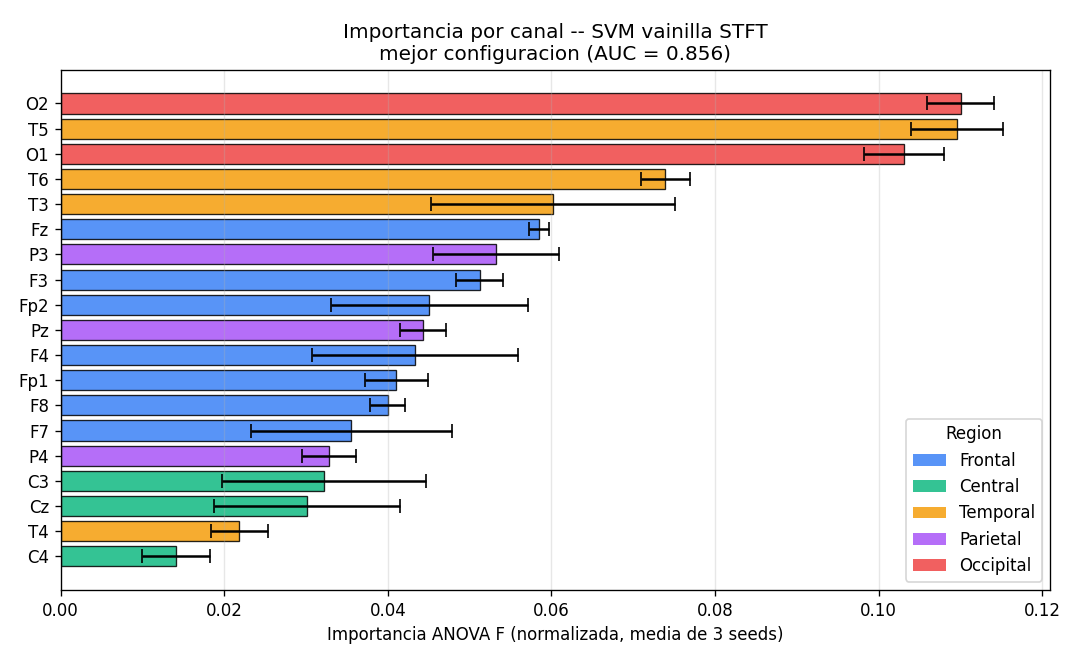
\includegraphics[width=0.85\textwidth]{figures_informe_final/channel_importance.png}
    \caption{Importancia por canal del SVM vainilla STFT
    (mejor configuración, AUC $= 0.856$).}
    \label{fig:channel_importance}
\end{figure}

\subsection{Consistencia de patches entre folds (Jaccard)}

Jaccard entre máscaras de patches de pares aleatorios de folds
(200~pares por configuración):

\begin{center}
\small
\begin{tabular}{lc}
\toprule
Configuración & Jaccard medio $\pm$ SD \\
\midrule
STFT Grad-CAM & $0.050$--$0.063$ \\
STFT vainilla & $0.036$--$0.051$ \\
CWT Grad-CAM  & $0.042$--$0.045$ \\
CWT vainilla  & $0.026$--$0.030$ \\
\bottomrule
\end{tabular}
\end{center}

\textbf{Los patches descubiertos son extremadamente inestables entre
folds} (Jaccard $\approx 0.03$--$0.06$). Esto matiza la narrativa de
``biomarcadores reproducibles'': cada fold descubre regiones distintas,
aunque las métricas globales sean buenas.

\subsection{Figura maestra}

\begin{figure}[H]
    \centering
    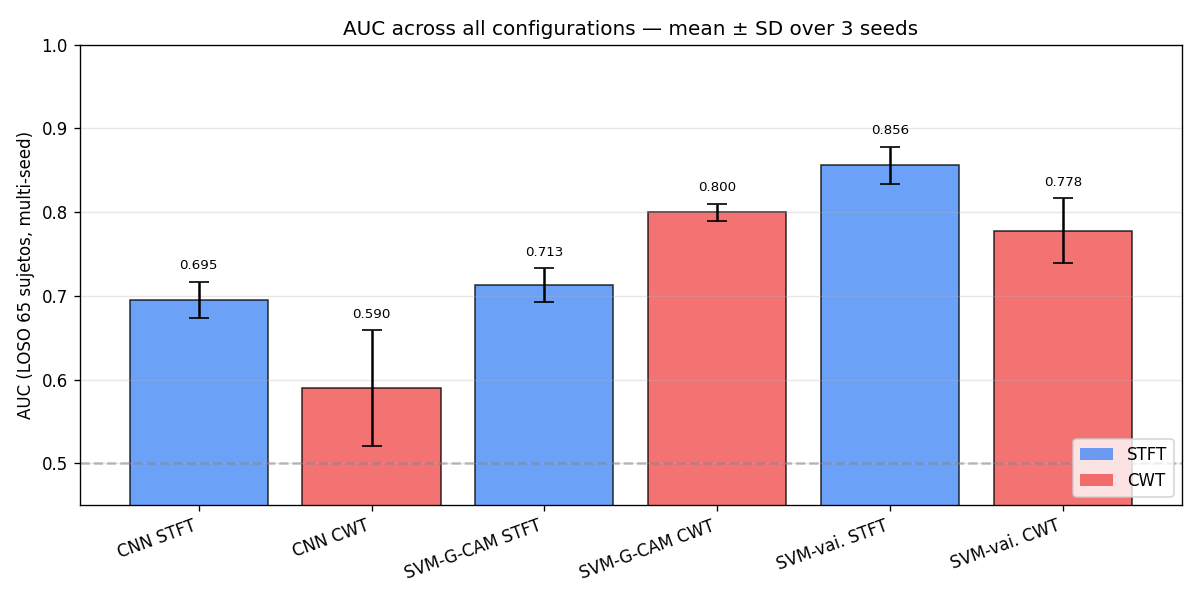
\includegraphics[width=0.95\textwidth]{figures_informe_final/auc_master_summary.png}
    \caption{Resumen visual de AUC por configuración, agregando las
    6~combinaciones (CNN/SVM vainilla/SVM Grad-CAM~$\times$~STFT/CWT)
    con error bars entre seeds. Mejor configuración: SVM vainilla STFT
    (AUC $= 0.856 \pm 0.022$).}
    \label{fig:auc_master}
\end{figure}

% =============================================================
\section{Discusión}
% =============================================================

\subsection{¿CWT supera a STFT?}
\label{sec:discusion_cwt}

\textbf{Respuesta: a igualdad de eje de modulación, STFT y CWT-Morlet
son estadísticamente indistinguibles.} Ni la hipótesis original
(CWT > STFT) ni la inversa obtienen soporte. Lo importante es \emph{cómo}
se llega a esa conclusión, porque una comparación ingenua (STFT vs CWT
nativa) engaña.

\textbf{El eje de modulación era un confound, y controlarlo lo
demuestra.} STFT (noverlap=64 a fs=200) tiene Nyquist de modulación
$\approx$1.56~Hz; la CWT nativa lo preserva a 100~Hz. La condición
\textbf{CWT-fair} iguala ese eje manteniendo idéntica la transformada de
portadora, separando los dos efectos:

\begin{table}[H]
\centering
\small
\begin{tabular}{lcccc}
\toprule
 & AUC vainilla & vs STFT & AUC Grad-CAM & vs STFT \\
\midrule
STFT & $0.856$ & --- & $0.713$ & --- \\
CWT nativa & $0.778$ & $-0.078$ ($p=0.061$) & $0.800$ & $+0.087$ \\
\textbf{CWT-fair} & $0.828$ & $\mathbf{-0.028}$ ($p=0.318$) & $0.769$ & $\mathbf{+0.056}$ ($p=0.587$) \\
\bottomrule
\end{tabular}
\end{table}

\textbf{El patrón es simétrico y contundente}: en vainilla la CWT nativa
parecía \emph{peor} que STFT y en Grad-CAM parecía \emph{mejor}; en
\textbf{ambos casos}, igualar el eje \textbf{mueve la CWT hacia la STFT}
(reduce $|\Delta$ AUC$|$ de 0.078$\to$0.028 y de 0.087$\to$0.056). Las
diferencias aparentes en las dos direcciones eran mayoritariamente el
\textbf{artefacto de DSP}, no la transformada. La comparación justa
(STFT vs CWT-fair) es no significativa en ambos métodos de saliency, y
también la CWT-nativa vs CWT-fair ($p=0.283, 0.527$).

\textbf{Matices que persisten} (acotan la generalización):

\begin{itemize}[leftmargin=*]
    \item \textbf{CWT-fair iguala ``hacia abajo''}: descarta las
    modulaciones rápidas ($>1.56$~Hz) de la CWT nativa. Es la elección
    conservadora y fisiológicamente razonable (AM diagnóstica lenta en
    EA; Fraga 2013). La alternativa (STFT con hop fino) se deja como
    trabajo futuro (§5.5).
    \item \textbf{Mayor varianza de la CWT} entre seeds (AUC
    $\pm 0.031$--$0.045$ fair vs $\pm 0.022$ STFT).
    \item \textbf{CWT con \texttt{cmor1.5-1.0}, 32~escalas log}, sin
    tuning específico; hiperparámetros del CNN optimizados por Lopes para
    input STFT.
\end{itemize}

\textbf{Lectura defendible}: \emph{bajo un eje de modulación equiparable,
la elección STFT vs CWT-Morlet no cambia el poder discriminativo de este
pipeline}. Es más fuerte y más honesto que el resultado ingenuo, porque
atribuye correctamente las diferencias a su causa (DSP), no a la
transformada.

\begin{figure}[H]
    \centering
    \begin{subfigure}{0.48\linewidth}
        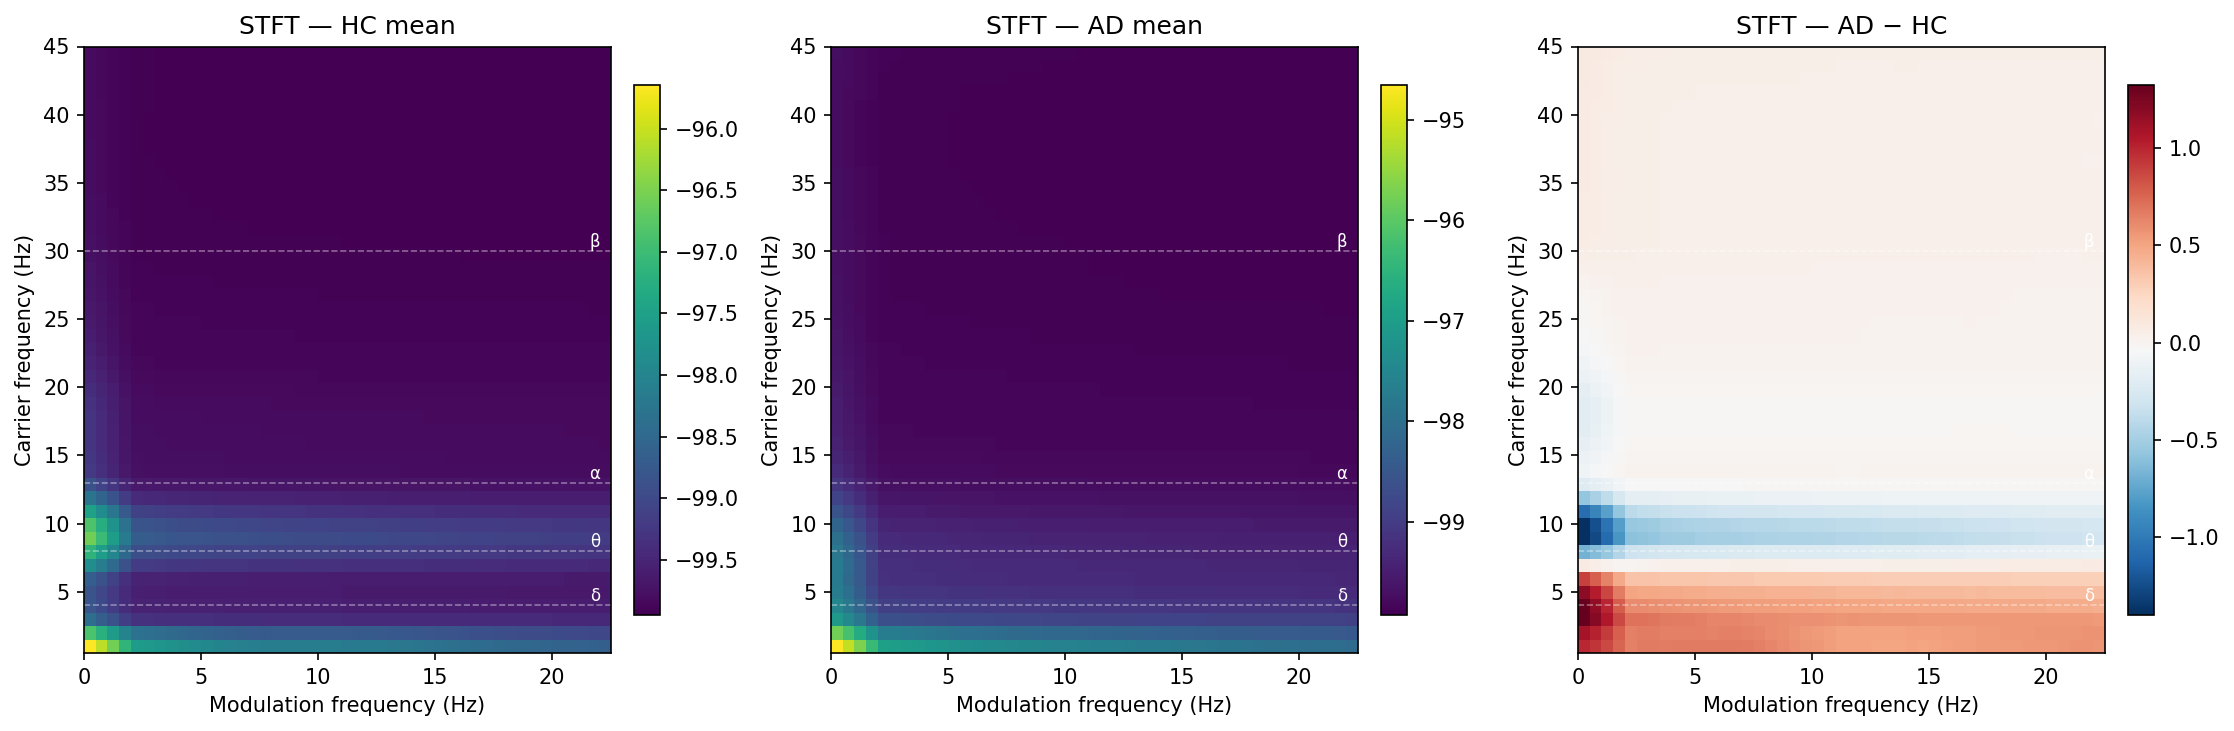
\includegraphics[width=\linewidth]{figures_informe_final/modspec_means_stft.png}
        \caption{STFT.}
    \end{subfigure}
    \hfill
    \begin{subfigure}{0.48\linewidth}
        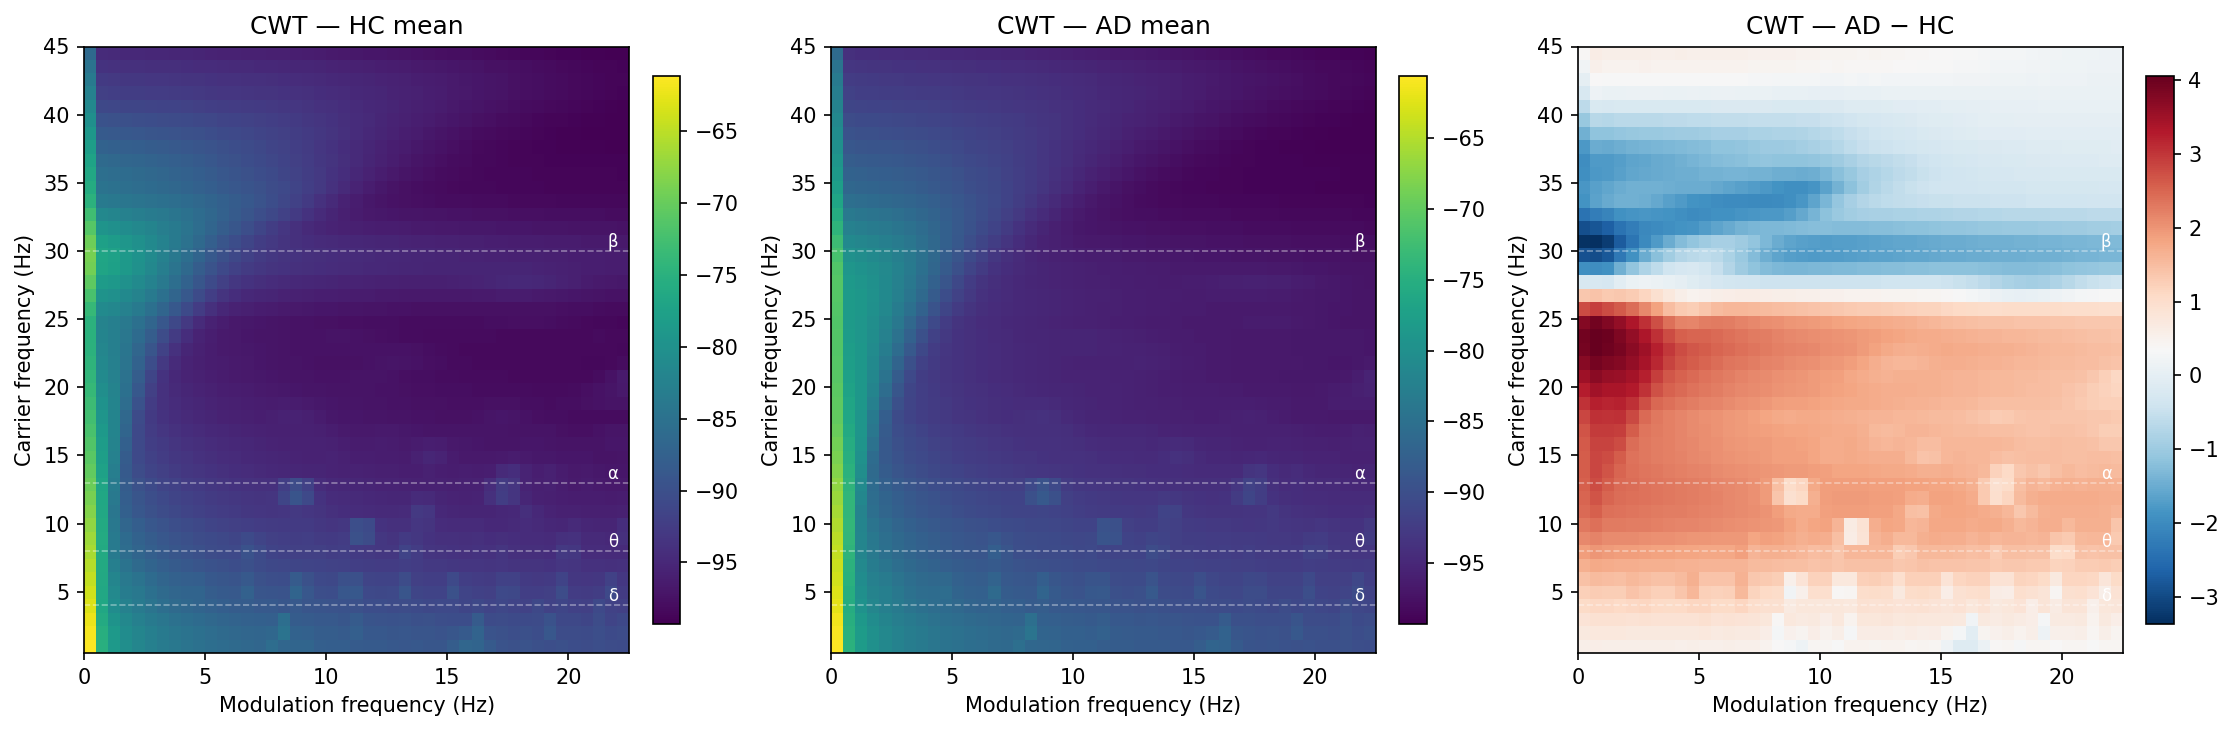
\includegraphics[width=\linewidth]{figures_informe_final/modspec_means_cwt.png}
        \caption{CWT-Morlet.}
    \end{subfigure}
    \caption{Espectrogramas de modulación promedio (AD vs HC) bajo STFT
    y CWT. La presentación $45\times45$ oculta el desajuste en el rango
    del eje de modulación (Nyquist $1.56$~Hz vs $100$~Hz).}
\end{figure}

\subsection{El método de saliency cambia el ranking}

\textbf{Hallazgo metodológico relevante}: con Grad-CAM, CWT tiende a
tener mejor AUC media; con vainilla (paper-faithful), STFT tiene mejor
AUC media. Los saliency maps de los dos métodos no se parecen
($r \approx 0.11$ STFT, $-0.17$ CWT), lo que indica que descubren
regiones distintas del espectrograma de modulación.

Esto implica que comparaciones del tipo ``transformada $X$ supera
transformada $Y$'' son sensibles al método de saliency y al pipeline
completo.

\begin{figure}[H]
    \centering
    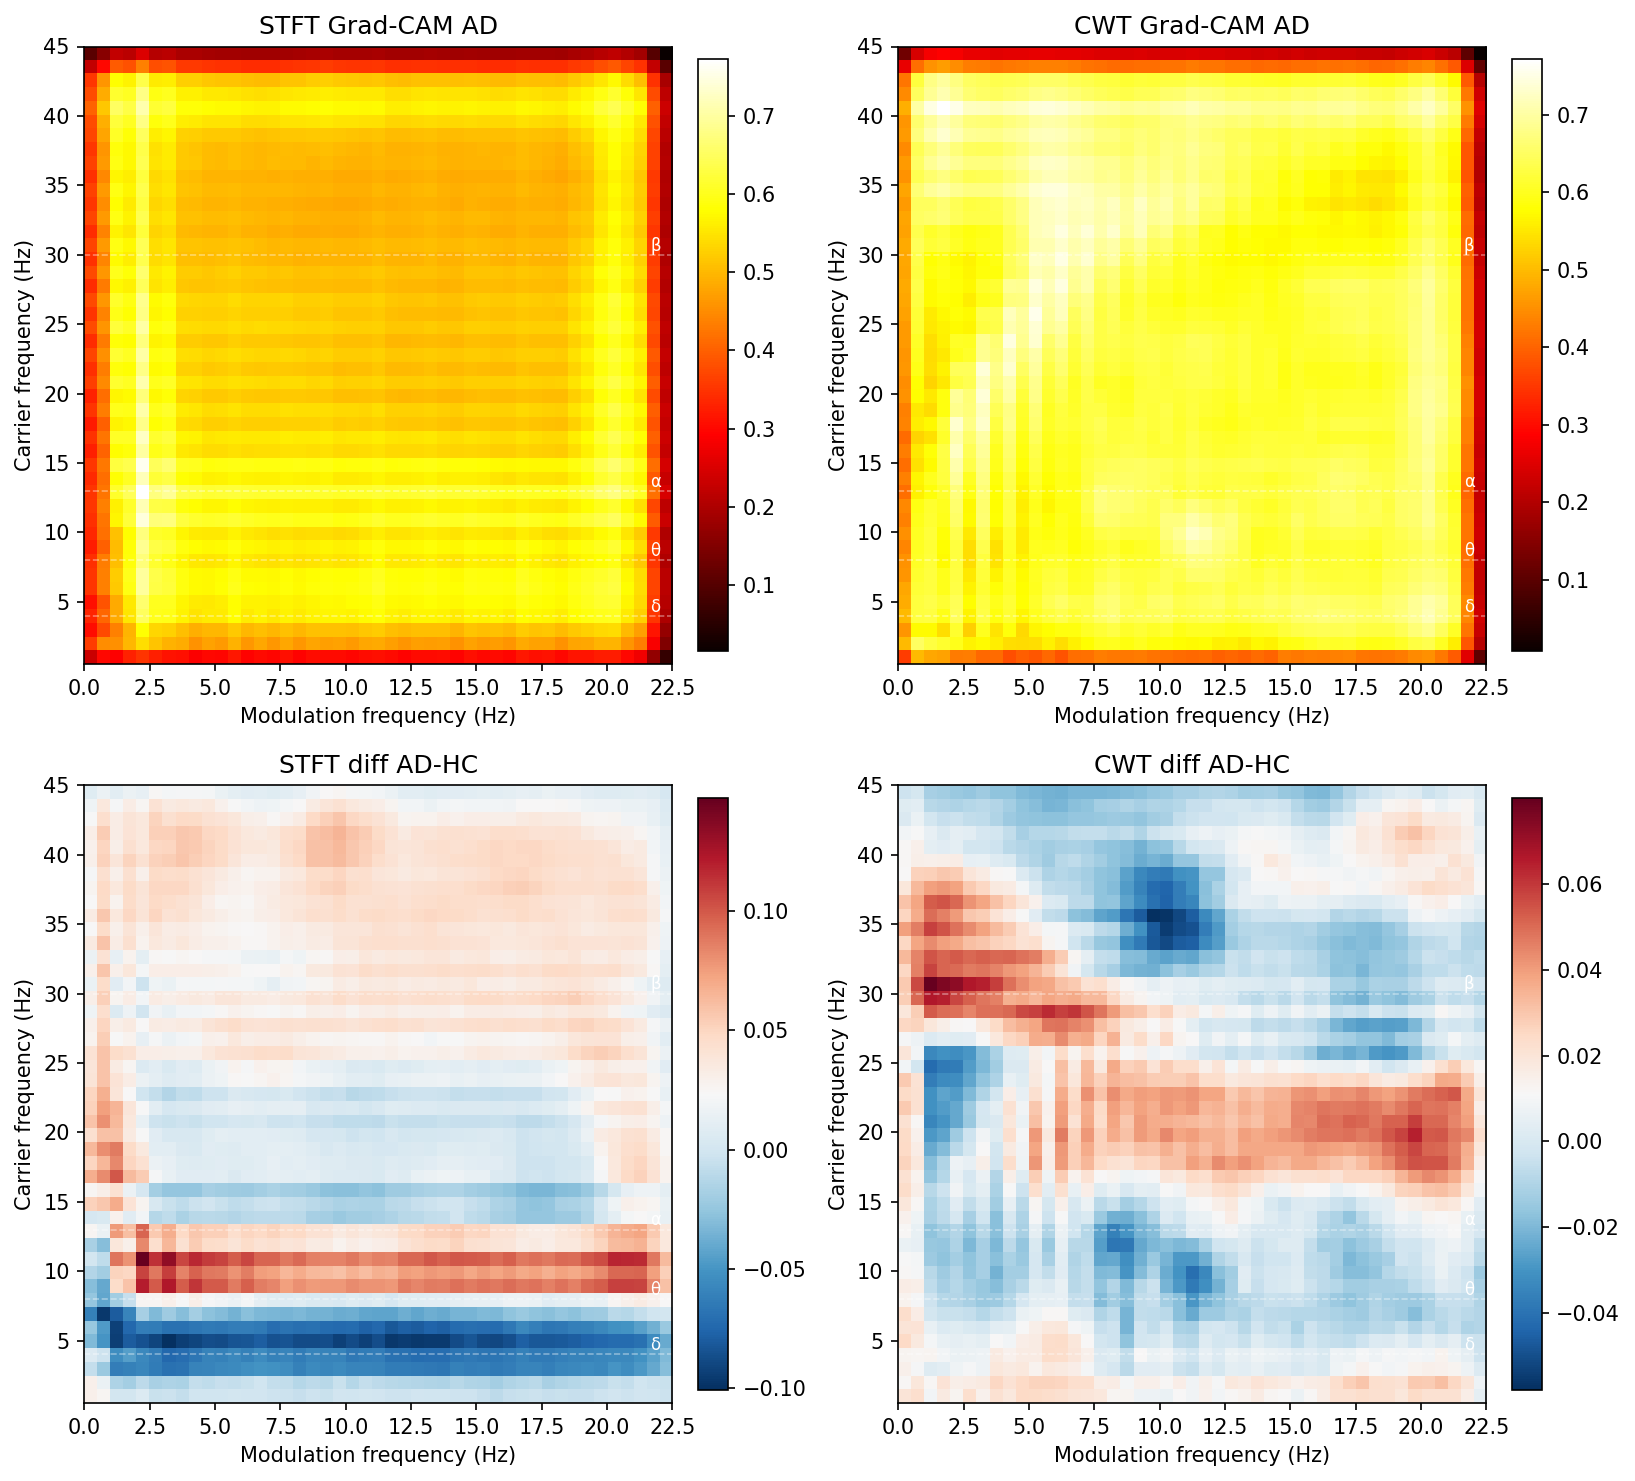
\includegraphics[width=0.95\textwidth]{figures_informe_final/saliency_compare.png}
    \caption{Comparación de saliency maps medios entre STFT y CWT bajo
    el método vainilla. Las distribuciones son cualitativamente
    distintas, coherente con Pearson $r \approx -0.09$.}
\end{figure}

\begin{figure}[H]
    \centering
    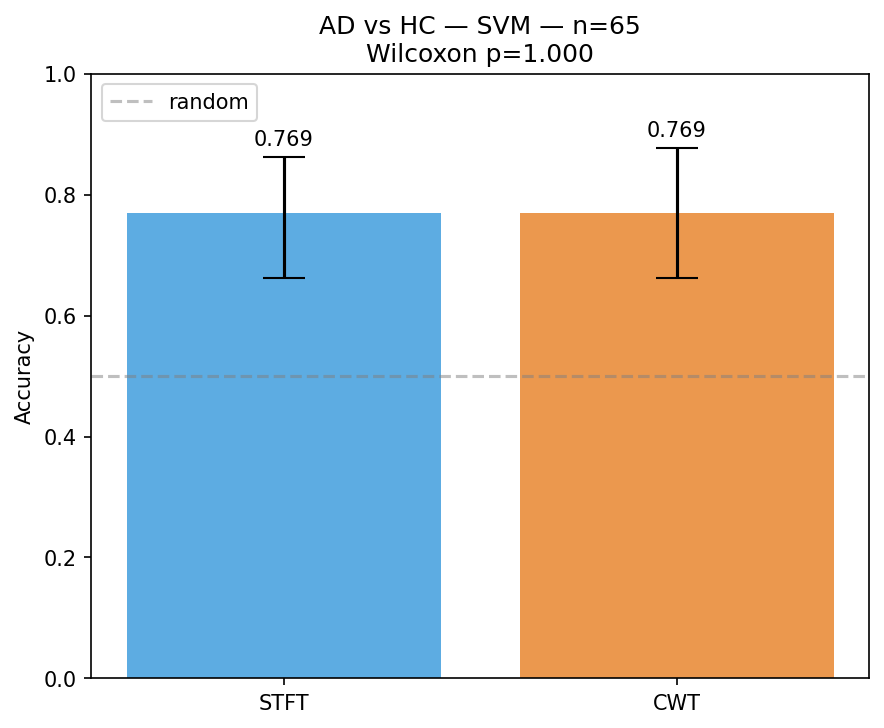
\includegraphics[width=0.95\textwidth]{figures_informe_final/compare_svm.png}
    \caption{Comparación cuantitativa SVM con saliency vainilla:
    STFT vs CWT por configuración.}
\end{figure}

\subsection{Replicación del paper}

Sobre \texttt{ds004504}, el SVM vainilla con STFT alcanza
$\text{Acc} = 0.764 \pm 0.009$, AUC $= 0.856 \pm 0.022$, en el mismo
orden de magnitud que el $0.71 \pm 0.02$ del paper en T2. La comparación
numérica es \textbf{orientativa, no estricta}: datasets, poblaciones y
detalles de anti-leakage difieren.

\begin{figure}[H]
    \centering
    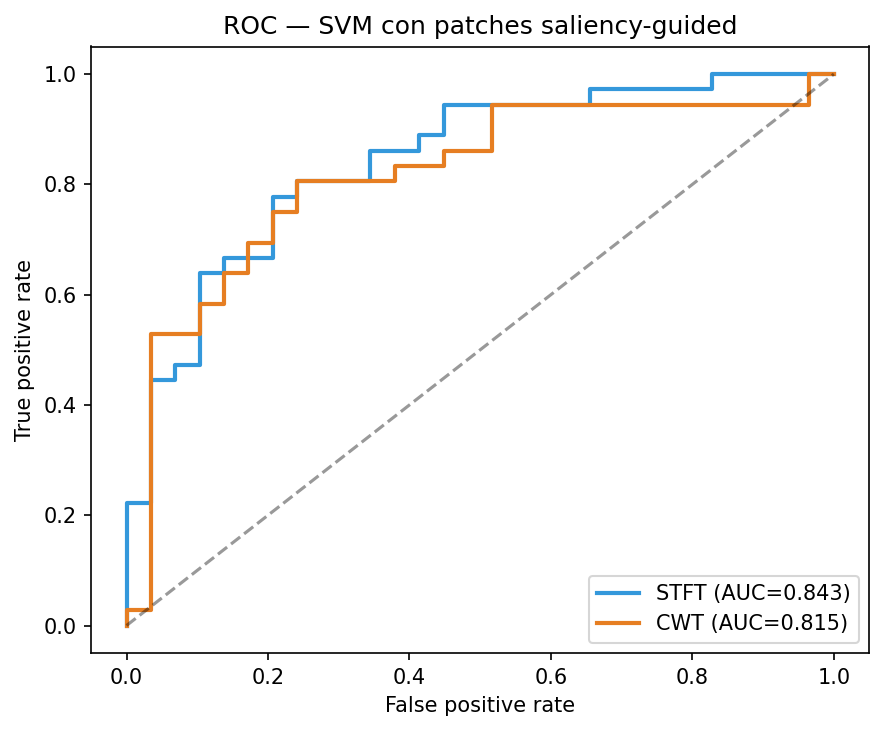
\includegraphics[width=0.85\textwidth]{figures_informe_final/roc_svm.png}
    \caption{Curva ROC del SVM con saliency vainilla, agregada sobre
    todos los sujetos (LOSO).}
\end{figure}

\subsection{Ensemble multi-seed y análisis estratificado por género}

\textbf{Ensemble}: agregando las 3~semillas con votación por mediana
(SVM vainilla STFT), la accuracy sube a $0.831$ y AUC a $0.900$.

\textbf{Análisis estratificado por género} (Fisher exact test sobre
clasificación correcta):

\begin{table}[H]
\centering
\small
\begin{tabular}{lccccc}
\toprule
Género & $n$ & AD/HC & Aciertos & Acc & AUC \\
\midrule
Mujer  & 35 & 24/11 & 27/35 & $0.771$ & $0.852$ \\
Hombre & 30 & 12/18 & 27/30 & $0.900$ & $0.940$ \\
Diferencia & --- & --- & --- & $\mathbf{+0.129}$ & $+0.088$ \\
Fisher exact F vs M & --- & --- & OR $\approx 0.375$ & $\mathbf{p = 0.201}$ & Cohen $h \approx 0.35$ \\
\bottomrule
\end{tabular}
\end{table}

\textbf{Análisis de poder estadístico}: con un tamaño de efecto Cohen
$h \approx 0.35$ (moderado), detectar la diferencia observada al 80\%
de poder y $\alpha = 0.05$ requeriría aproximadamente
$N \approx 64$~sujetos por grupo (es decir, $\sim 129$~sujetos totales
sumando F y M), según la fórmula con transformación arcoseno:
$n_{\text{grupo}} = ((z_{1-\alpha/2} + z_{1-\beta})/h)^2 \approx 64$.
El tamaño actual (35F + 30M) tiene poder $\sim 25$--$30\%$ para esa
diferencia.

\textbf{Lectura prudente}: no se detectó diferencia significativa entre
géneros, pero el poder estadístico es limitado — la diferencia absoluta
de 12.9~puntos en accuracy es relevante en magnitud, y no podemos
descartar un sesgo real del modelo. \textbf{Ausencia de evidencia
no es evidencia de ausencia}.

\subsection{Limitaciones}
\label{sec:limitaciones}

\begin{enumerate}[leftmargin=*]
    \item \textbf{Solo 3 seeds}: el multi-seed reporta varianza pero el
    número de réplicas es bajo para inferencias estadísticas fuertes.
    Idealmente $\geq 10$~seeds.
    \item \textbf{Grid search de patches heurístico, no nested CV}:
    selección por separabilidad de saliency map, no validación con
    SVM en val set.
    \item \textbf{BH-FDR post-hoc}: la corrección se aplicó después de
    ver los resultados, no como pre-registro. Ninguna comparación justa
    (STFT vs CWT-fair) se acerca a la significancia ($q \geq 0.58$).
    \item \textbf{CWT-fair ``iguala hacia abajo'' el eje de modulación}:
    decima la envolvente a 3.125~Hz, descartando modulaciones $>1.56$~Hz
    de la CWT nativa. Es la definición \emph{conservadora} de ``justo''
    (y fisiológicamente razonable), pero no única; la alternativa
    (igualar ``hacia arriba'' con STFT de hop fino) queda como futuro.
    Por eso la conclusión es ``a igualdad de eje de modulación
    \emph{lento}''.
    \item \textbf{Resize bilinear}: tras igualar el eje (CWT-fair), STFT
    y CWT-fair parten de $\sim$13 bins reales interpolados a 45, así que
    el resize ya no introduce asimetría entre ellas; la CWT nativa sí
    quedaba subsampleada.
    \item \textbf{CWT subexplorada}: solo \texttt{cmor1.5-1.0} con
    32~escalas log; sin cone-of-influence; sin tuning específico.
    \item \textbf{Resolución STFT real $\neq$ nominal}:
    $\Delta f = 1.5625$~Hz, no 1~Hz exacto.
    \item \textbf{Inferencia entre seeds con solo 3 réplicas}: DeLong por
    seed + combinación (Stouffer/Fisher) es correcto pero de potencia
    limitada; un modelo de efectos mixtos con $\geq 10$ seeds sería más
    robusto.
    \item \textbf{CNN sub-entrenada}: dropout 0.85 muy agresivo.
    \item \textbf{Sin validación externa}: solo \texttt{ds004504}.
    \item \textbf{Tareas binarias solamente}: el paper original tiene
    5~tareas (T1--T5); este TFM replica solo T2.
    \item \textbf{Poder estadístico modesto} para sub-análisis (género
    $N = 65$, potencia $\sim 25$--$30\%$ para $h \approx 0.35$).
    \item \textbf{Saliency unstable fold-to-fold} (Jaccard $\approx 0.05$).
    \item \textbf{Atribución de bandas canónicas restringida a STFT}:
    eje portador CWT (\texttt{geomspace}) requiere mapeo distinto.
    \item \textbf{$N$ efectivo por autocorrelación de epochs}: el
    overlap 87.5\% intra-sujeto NO afecta los tests reportados porque
    todas las inferencias finales son a nivel de sujeto.
    \item \textbf{Análisis post-hoc} (bandas, importancia por canal,
    correlaciones, género) no estaban pre-registrados; deben verse como
    exploratorios.
\end{enumerate}

\subsection{Aporte propio}

Más allá de la replicación, este TFM aporta:

\begin{enumerate}[leftmargin=*]
    \item \textbf{Evaluación multi-seed} del pipeline (el paper original
    no reporta varianza por seed). Aquí se cuantifica.
    \item \textbf{Comparación STFT vs CWT controlando el confound DSP del
    eje de modulación} --- el aporte metodológico central. Se identifica
    que STFT y CWT nativa tienen ejes de modulación no equiparables, se
    introduce la condición \textbf{CWT-fair} que los iguala, y se
    demuestra que las diferencias aparentes (en ambas direcciones y
    ambos métodos de saliency) eran ese artefacto: a igualdad de eje, las
    transformadas son indistinguibles (DeLong + Stouffer + BH-FDR).
    \item \textbf{Observación de pipeline-dependencia y su origen}: el
    método de saliency cambia el ranking aparente entre STFT y CWT
    nativa, pero la sensibilidad se atenúa al controlar el eje.
    \item \textbf{Conexión exploratoria con literatura clínica}:
    STFT~+~vainilla concentra saliency en bandas $\alpha + \theta$ y
    canales occipito-temporales.
    \item \textbf{Auditoría DSP + ML documentada} y validada por dos
    rondas de revisión externa + revisión adversarial multi-agente del
    código del fix.
    \item \textbf{Reproducibilidad total}: repo público con
    \texttt{requirements-lock.txt}, seeds fijas, configs YAML, tests
    unitarios pasando.
\end{enumerate}

% =============================================================
\section{Conclusiones}
% =============================================================

\begin{enumerate}[leftmargin=*]
    \item \textbf{El pipeline de Lopes et al.~2023 fue replicado
    funcionalmente} sobre el dataset público \texttt{ds004504}. SVM con
    saliency vainilla y STFT alcanza Acc $= 0.764 \pm 0.009$,
    AUC $= 0.856 \pm 0.022$ (3~seeds), en el orden de magnitud del
    $0.71 \pm 0.02$ reportado por Lopes en T2.

    \item \textbf{A igualdad de eje de modulación, STFT y CWT-Morlet son
    estadísticamente indistinguibles; las diferencias aparentes eran un
    artefacto de DSP.} STFT (Nyquist de modulación 1.56~Hz) y CWT nativa
    (100~Hz) no codifican el mismo eje vertical antes del resize. La
    condición de control \textbf{CWT-fair} muestra:
    \begin{itemize}[leftmargin=*]
        \item Con \emph{vainilla}, la CWT pasa de $-0.078$ AUC vs STFT
        (nativa, $p=0.061$) a $\mathbf{-0.028}$ (fair, $p=0.318$).
        \item Con \emph{Grad-CAM}, de $+0.087$ (nativa) a $\mathbf{+0.056}$
        (fair, $p=0.587$).
        \item En \textbf{ambas direcciones} igualar el eje mueve la CWT
        hacia la STFT; ninguna comparación justa sobrevive BH-FDR
        ($q \geq 0.58$). \textbf{La elección STFT vs CWT-Morlet no cambia
        el desempeño una vez controlado el eje.}
    \end{itemize}

    \item \textbf{La sensibilidad del ranking al método de saliency
    también era, en parte, el confound}: con CWT nativa el ranking se
    invierte (Grad-CAM: CWT mejor; vainilla: STFT mejor); esa inversión
    se atenúa con CWT-fair. Los saliency maps STFT$\leftrightarrow$CWT
    son \textbf{estadísticamente ortogonales} ($r \approx -0.09$
    vainilla, $-0.24$ Grad-CAM) --- descubren regiones distintas, pero
    ello no se traduce en diferencia de desempeño con el eje igualado.

    \item \textbf{Observaciones exploratorias (post-hoc)}:
    STFT~+~vainilla concentra saliency en bandas $\alpha$~(61\%)~+
    $\theta$~(28\%) y canales occipito-temporales (O1, O2, T5, T6),
    coherente con biomarcadores clásicos de EA. Requiere validación en
    datasets independientes.

    \item \textbf{Hallazgos metodológicos para la comunidad}:
    \begin{itemize}[leftmargin=*]
        \item \textbf{Comparar representaciones T-F exige igualar el eje
        de modulación}: diferencias de resolución temporal nativa crean
        un confound que puede invertir el ranking aparente. CWT-fair es
        un control replicable.
        \item El método de saliency afecta las conclusiones
        cuantitativas; reportar siempre el método específico.
        \item Patches saliency-guided inestables entre folds (Jaccard
        $\approx 0.05$): matizar ``biomarcadores reproducibles''.
        \item Reportar varianza por seed y poder estadístico es esencial.
    \end{itemize}

    \item \textbf{Recomendaciones para trabajos futuros}:
    \begin{itemize}[leftmargin=*]
        \item Igualar el eje ``hacia arriba'' (STFT con hop fino) para
        ver si las modulaciones rápidas ($>1.56$~Hz) que CWT-fair
        descarta aportan poder discriminativo.
        \item CWT tuning específico (cmor1-1, $n_\text{scales}$ mayor,
        cone-of-influence).
        \item Ensemble STFT~+~CWT (late fusion) explotando ortogonalidad.
        \item Test externo en otro dataset EEG-AD.
        \item Banco de filtros con bandas no uniformes.
        \item Nested CV para grid search; dataset balanceado por género;
        $\geq 10$ seeds.
    \end{itemize}
\end{enumerate}

% =============================================================
\section{Reproducibilidad}
% =============================================================

\textbf{Repositorio}: \url{https://github.com/spalaciobe/tps-alzheimer-modspec}

\textbf{Para reproducir}:
\begin{lstlisting}[language=bash]
git clone https://github.com/spalaciobe/tps-alzheimer-modspec.git
cd tps-alzheimer-modspec
python -m venv .venv && source .venv/Scripts/activate
pip install -r requirements-lock.txt && pip install -e .
python scripts/00_download_dataset.py
bash scripts/run_remaining_v2.sh
\end{lstlisting}

\textbf{Tiempos en RTX~3050 Laptop (4~GB)}:

\begin{itemize}[leftmargin=*, itemsep=0pt]
    \item Preproceso 65 sujetos: $\sim$35~min.
    \item Modspecs (STFT + CWT): $\sim$90~min.
    \item LOSO CNN $\times$ 3~seeds $\times$ 2~métodos: $\sim$14~h.
    \item Saliency $\times$ 12~corridas: $\sim$12~h.
    \item SVM $\times$ 12~corridas: $\sim$12~h.
    \item Post-análisis + figuras: $\sim$30~min.
\end{itemize}

\textbf{Total}: $\sim$48~h de cómputo continuo. \\
\textbf{Stack}: Python 3.13, PyTorch 2.6+cu124, MNE 1.12,
scikit-learn 1.8.

% =============================================================
\section*{Declaración de uso de IA}
% =============================================================

La estructura del pipeline, scripts de orquestación, debugging de
leakage en LOSO-CV, refactor de optimización
(\texttt{SubjectBank}, fp16-bank, GC entre folds), auditoría
metodológica multi-dimensional y redacción de este informe fueron
asistidos por \textbf{Claude Code} (Anthropic) [Opus~4.7, 2026]. Todo el
código fue revisado, ejecutado y validado por el autor antes de cada
commit.

% =============================================================
% Bibliografía
% =============================================================
\begin{thebibliography}{99}

\bibitem{Lopes2023}
M.~Lopes, R.~Cassani, T.~H.~Falk.
\newblock Using CNN saliency maps and EEG modulation spectra for
improved and more interpretable machine learning-based Alzheimer's
disease diagnosis.
\newblock \emph{Computational Intelligence and Neuroscience}, vol. 2023,
art.~3198066, 2023. DOI:
\href{https://doi.org/10.1155/2023/3198066}{10.1155/2023/3198066}.

\bibitem{Miltiadous2023}
A.~Miltiadous \emph{et al.}
\newblock A dataset of scalp EEG recordings of Alzheimer's disease,
frontotemporal dementia and healthy subjects from routine EEG.
\newblock OpenNeuro \texttt{ds004504}, CC0~1.0, 2023.

\bibitem{Trambaiolli2011}
L.~R.~Trambaiolli \emph{et al.}
\newblock EEG spectro-temporal modulation energy: A new feature for
automated diagnosis of Alzheimer's disease.
\newblock \emph{IEEE EMBC}, pp.~3828--3831, 2011.

\bibitem{Fraga2013}
F.~J.~Fraga \emph{et al.}
\newblock Characterizing Alzheimer's disease severity via resting-awake
EEG amplitude modulation analysis.
\newblock \emph{PLoS ONE}, vol.~8, no.~8, e72240, 2013.

\bibitem{Cassani2020}
R.~Cassani, T.~H.~Falk.
\newblock Alzheimer's disease diagnosis and severity level detection
based on EEG modulation spectral `patch' features.
\newblock \emph{IEEE J. Biomed. Health Inform.}, vol.~24, no.~7,
pp.~1982--1993, 2020.

\bibitem{Selvaraju2017}
R.~R.~Selvaraju \emph{et al.}
\newblock Grad-CAM: Visual explanations from deep networks via
gradient-based localization.
\newblock \emph{ICCV}, 2017.

\bibitem{Simonyan2014}
K.~Simonyan, A.~Vedaldi, A.~Zisserman.
\newblock Deep inside convolutional networks: Visualising image
classification models and saliency maps.
\newblock \emph{ICLR Workshop}, 2014.

\bibitem{PionTonachini2019}
L.~Pion-Tonachini, K.~Kreutz-Delgado, S.~Makeig.
\newblock ICLabel: An automated electroencephalographic independent
component classifier.
\newblock \emph{NeuroImage}, vol.~198, pp.~181--197, 2019.

\bibitem{Gramfort2013}
A.~Gramfort \emph{et al.}
\newblock MEG and EEG data analysis with MNE-Python.
\newblock \emph{Frontiers in Neuroscience}, vol.~7, no.~267, 2013.

\bibitem{WHO2023}
World Health Organization.
\newblock Dementia fact sheet, 2023.
\newblock \url{https://www.who.int/news-room/fact-sheets/detail/dementia}

\end{thebibliography}

\end{document}
